\chapter{Groups}

Any user can create/modify a Group of users. A Group is a set of users identified by a name tag.
A Group belong to an individual user (who is the owner of the Group) and not visible to others.
If sharing is done frequently with a specific set of users, it is probably helpful to create a Group for 
those users. This will make it easy to share with the Group once instead of sharing separately with each of the 
individual users.

\section{Creating a Group}

\begin{figure}[H]
\centering
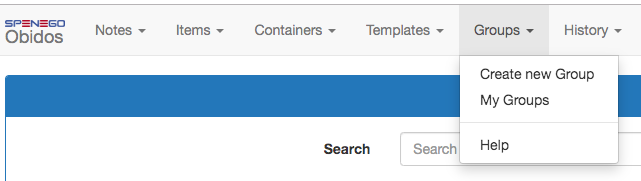
\includegraphics[scale=0.4]{user/Create-Group-Menu.png}
\caption{Creating a Group}
\label{fig: Figure}
\end{figure}

\begin{figure}[H]
\centering
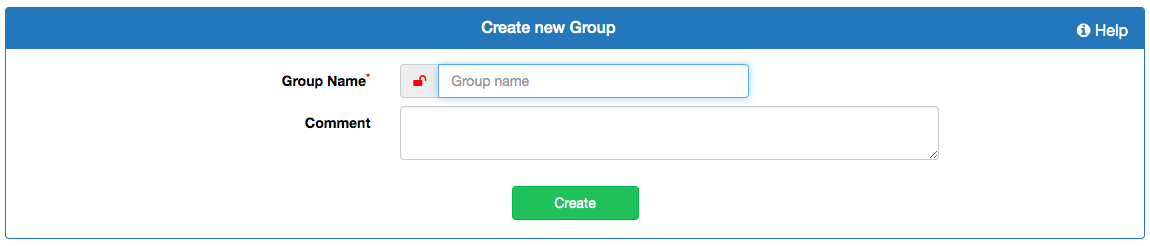
\includegraphics[scale=0.4]{user/Create-Group.png}
\caption{Creating a Group}
\label{fig: Figure}
\end{figure}

\section{Adding Users to a Group}

\begin{figure}[H]
\centering
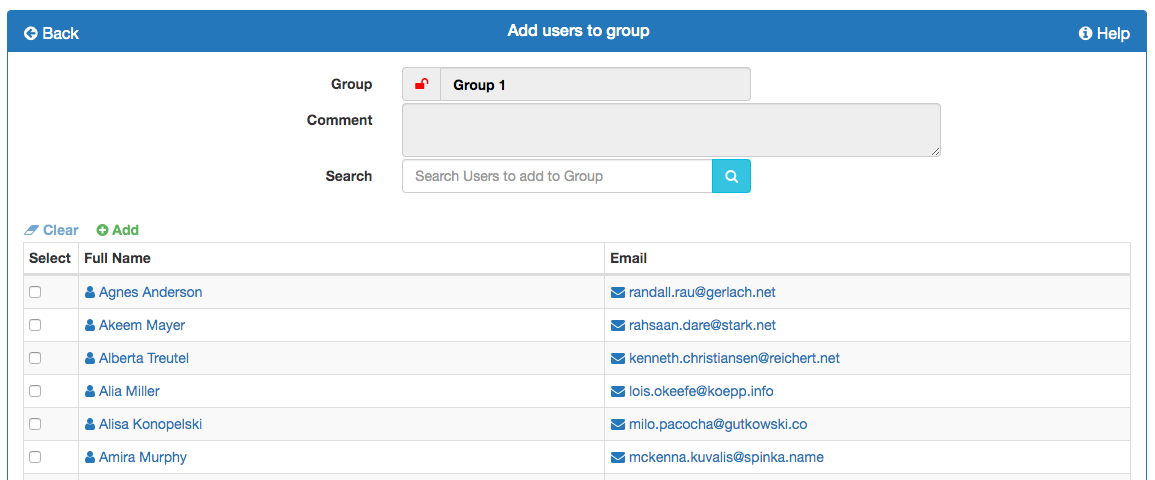
\includegraphics[scale=0.4]{user/Add-Users-to-Group.png}
\caption{Add Users to a Group}
\label{fig: Figure}
\end{figure}

\section{Deleting Users From a Group}

\begin{figure}[H]
\centering
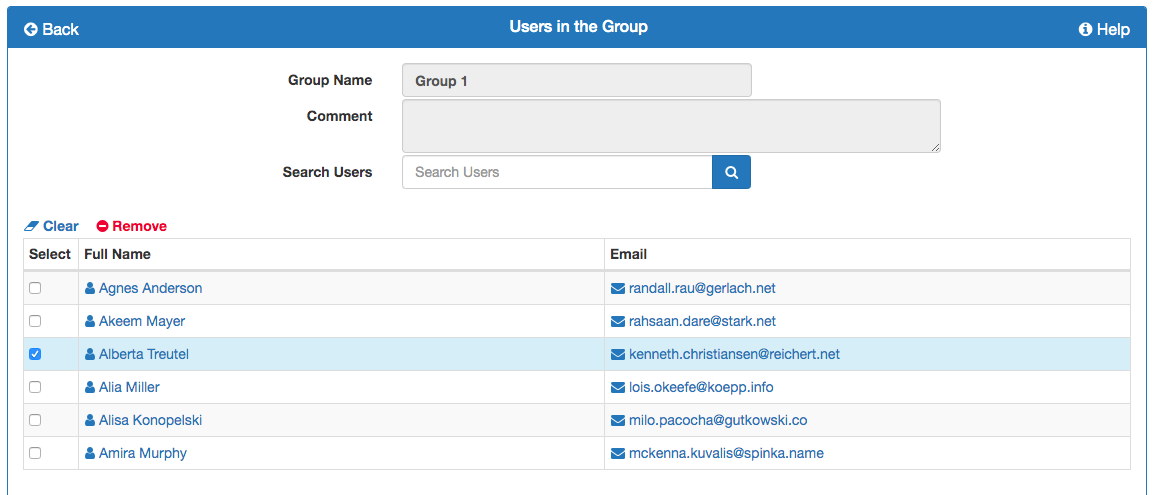
\includegraphics[scale=0.4]{user/Delete-Users-from-Group.png}
\caption{Listing Groups}
\label{fig: Figure}
\end{figure}

\section{Changing Group name}

\begin{figure}[H]
\centering
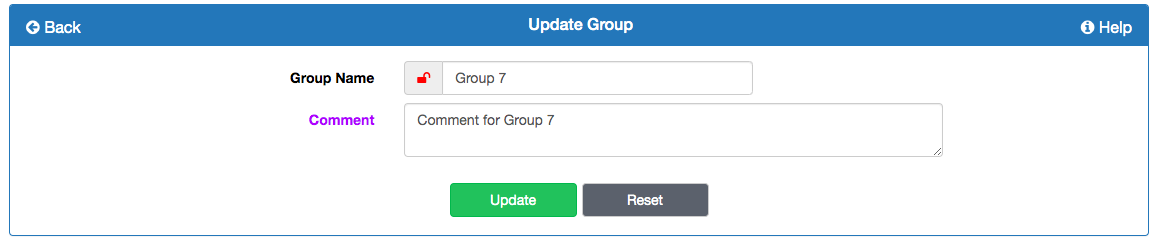
\includegraphics[scale=0.4]{user/Change-Group-Name.png}
\caption{Changing a Group Name}
\label{fig: Figure}
\end{figure}

\section{Listing Groups}

\begin{figure}[H]
\centering
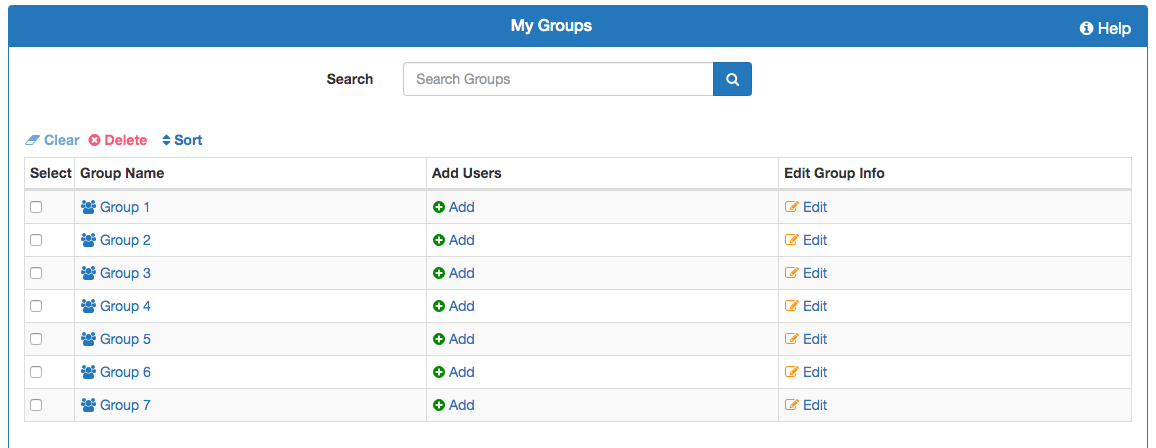
\includegraphics[scale=0.4]{user/Listing-Groups.png}
\caption{Listing Groups}
\label{fig: Figure}
\end{figure}

